\documentclass[10pt,a4paper]{article}

\usepackage[utf8]{inputenc}
\usepackage[T1]{fontenc}
\usepackage[dutch]{babel}
\usepackage{amsmath}
\usepackage{graphicx}
\usepackage{booktabs}
\usepackage{float}
\usepackage{geometry}
\usepackage{caption}

\geometry{margin=1.8cm}
\setlength{\parindent}{0pt}
\setlength{\parskip}{0.45em}
\captionsetup{font=small,labelfont=bf}

\title{Project Elementaire Statistiek}
\author{Voornaam Achternaam\\Studentennummer: 20246031}
\date{}

\begin{document}
\maketitle
\vspace{-1.5em}

Voor alle onderdelen werd gewerkt met significantieniveau $\alpha = 0.01$. De datasets werden in R ingelezen en daarna werden de persoonlijke steekproeven gemaakt met mijn studentennummer als seed. Ik gebruik enkel methodes uit de cursus: kruistabellen met een chi-kwadraattoets, lineaire regressie en een eenzijdige t-toets.

\section{Sneeuwcondities}

De drie variabelen zijn discreet, dus ik werk met een driedimensionale kruistabel. Omdat gevraagd wordt om \'{e}\'{e}n globale test te gebruiken, test ik niet elk paar afzonderlijk. De nulhypothese is volledige onderlinge onafhankelijkheid van temperatuurklasse, sneeuwtype en lawine-alarm. Onder deze hypothese worden de verwachte frequenties berekend uit de marginale verdelingen. De gebruikte teststatistiek is
\[
X^2 = \sum \dfrac{(O-E)^2}{E},
\]
waarbij $O$ de waargenomen frequentie is en $E$ de verwachte frequentie onder onafhankelijkheid. Er zijn $3\cdot2\cdot2=12$ cellen. Omdat de drie marginale verdelingen geschat worden, is het aantal vrijheidsgraden
\[
12-1-((3-1)+(2-1)+(2-1))=7.
\]

\begin{figure}[H]
    \centering
    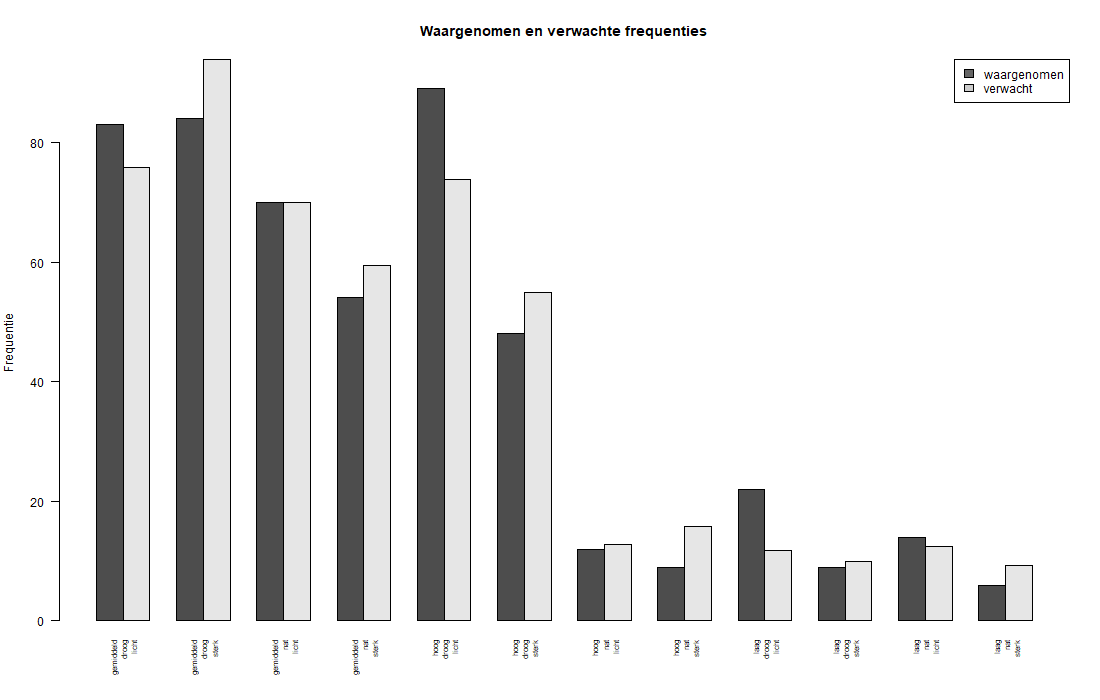
\includegraphics[width=0.83\textwidth]{figuren/sneeuw_waargenomen_verwacht.png}
    \caption{Waargenomen en verwachte frequenties voor de sneeuwdata.}
\end{figure}

De chi-kwadraatstatistiek is $X^2=19.5721$ en de kritieke waarde op het $1\%$-niveau is $18.4753$. De p-waarde is $0.00657$. De kleinste verwachte frequentie is $9.25$, dus de chi-kwadraatbenadering is voldoende bruikbaar. Omdat $19.5721>18.4753$ en $0.00657<0.01$, verwerp ik $H_0$. Er is dus op het $1\%$-niveau voldoende bewijs dat de drie variabelen niet volledig onderling onafhankelijk zijn. Dit betekent niet automatisch dat elk paar apart afhankelijk is, maar wel dat de gezamenlijke verdeling niet past bij volledige onafhankelijkheid.

\section{Temperatuur}

Voor de temperatuurmetingen onderzoek ik of de temperatuur voorspeld kan worden met hoogte en afstand tot de vallei. De correlatie tussen hoogte en temperatuur is sterk negatief ($r=-0.798$), wat logisch is: hogere plaatsen zijn gemiddeld kouder. De gewone correlatie tussen afstand tot de vallei en temperatuur is klein ($r=0.0367$), maar in een meervoudig regressiemodel kan deze variabele toch nuttig zijn wanneer de hoogte constant gehouden wordt.

Ik schat het lineaire model
\[
\text{Temperatuur}=\beta_0+\beta_1\cdot\text{Hoogte}+\beta_2\cdot\text{Afstand tot vallei}+\varepsilon.
\]
Dit geeft als geschatte vergelijking
\[
\widehat{\text{Temperatuur}}=43.1734-0.04555\cdot\text{Hoogte}+1.2518\cdot\text{Afstand tot vallei}.
\]
Bij gelijke afstand tot de vallei komt $100$ meter extra hoogte dus overeen met ongeveer $4.55^\circ$C lagere voorspelde temperatuur. Bij gelijke hoogte komt $1$ km extra afstand tot de vallei overeen met ongeveer $1.25^\circ$C hogere voorspelde temperatuur.

\begin{table}[H]
\centering
\small
\begin{tabular}{lrrr}
\toprule
Variabele & Schatting & p-waarde & $99\%$-BI \\
\midrule
Intercept & $43.1734$ & $<2\cdot10^{-16}$ & $[40.7816,45.5652]$ \\
Hoogte & $-0.04555$ & $<2\cdot10^{-16}$ & $[-0.04802,-0.04307]$ \\
Afstand tot vallei & $1.2518$ & $<2\cdot10^{-16}$ & $[1.1265,1.3771]$ \\
\bottomrule
\end{tabular}
\caption{Geschatte co\"effici\"enten van het regressiemodel.}
\end{table}

Beide verklarende variabelen zijn significant op het $1\%$-niveau. Ook de globale F-test is zeer significant ($p<2.2\cdot10^{-16}$), dus het model is duidelijk beter dan een model zonder verklarende variabelen. De verklaarde variantie is hoog: $R^2=0.9024$ en de aangepaste $R^2=0.9016$. De residual standard error is $1.30^\circ$C, de RMSE is $1.293^\circ$C en de MAE is $1.042^\circ$C. De typische fout ligt dus ongeveer tussen $1$ en $1.3^\circ$C.

\begin{figure}[H]
    \centering
    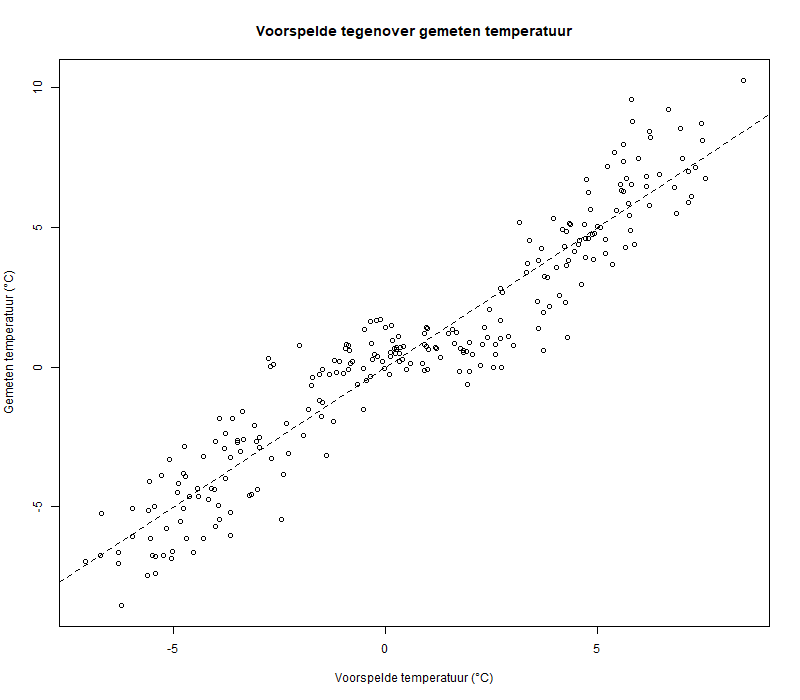
\includegraphics[width=0.63\textwidth]{figuren/temperatuur_voorspeld_observeerd.png}
    \caption{Voorspelde temperatuur tegenover gemeten temperatuur.}
\end{figure}

De punten liggen vrij dicht rond de diagonale lijn. Dat bevestigt dat het model op deze data goede voorspellingen maakt. De diagnosegrafieken uit R tonen geen perfect model, maar de QQ-plot van de residuen is redelijk lineair en de voorspelfout blijft beperkt. Daarom besluit ik dat temperatuur goed voorspeld kan worden aan de hand van hoogte en afstand tot de vallei.

\section{Wind}

Voor de winddata test ik of de gemiddelde windsnelheid groter is dan $11.7$ km/h. Omdat de variantie onbekend is, gebruik ik een eenzijdige t-toets voor \'{e}\'{e}n gemiddelde:
\[
H_0:\mu=11.7 \qquad \text{tegenover} \qquad H_1:\mu>11.7.
\]
De steekproef bevat $600$ observaties. Het gemiddelde is $62.168$ km/h en de standaardafwijking is $500.967$ km/h, terwijl de mediaan maar $11.889$ km/h is. Dat verschil wijst meteen op extreme waarden die het gemiddelde sterk omhoog trekken.

\begin{figure}[H]
    \centering
    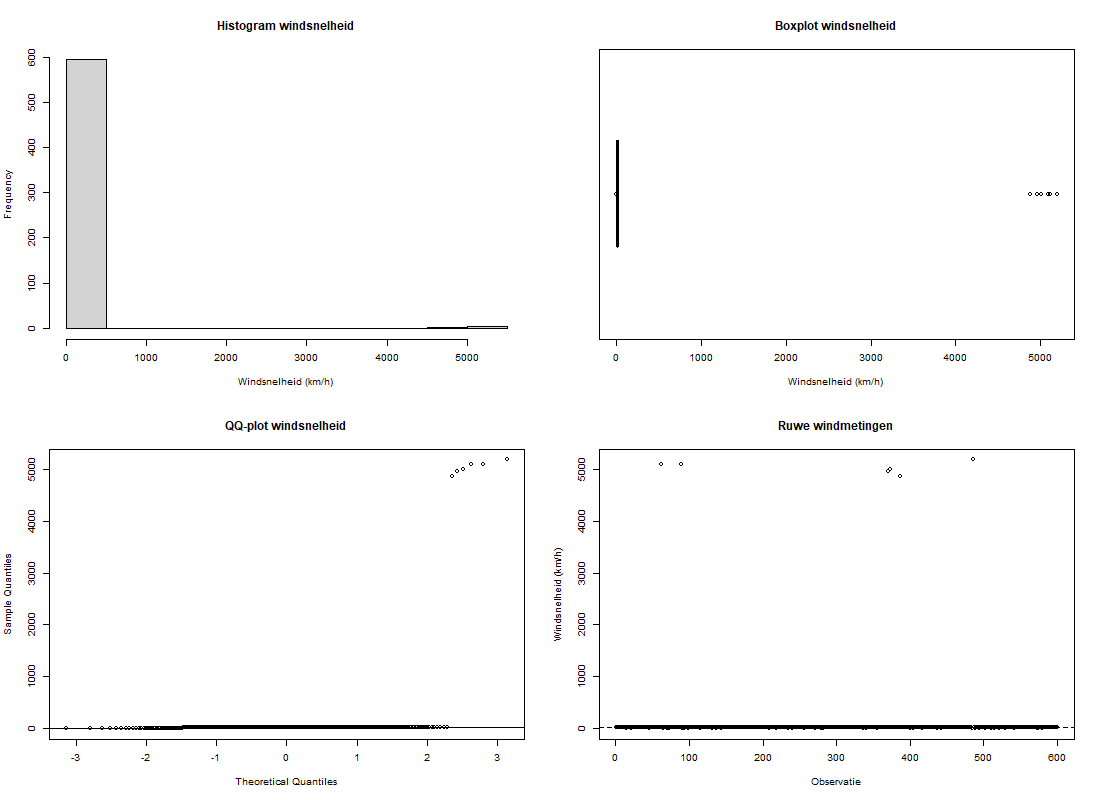
\includegraphics[width=0.72\textwidth]{figuren/wind_verkenning.png}
    \caption{Verkennende grafieken voor de windsnelheid.}
\end{figure}

In de grafieken zijn enkele waarden rond $5000$ km/h zichtbaar. Die zijn fysisch niet realistisch als gewone windsnelheid, dus ze lijken op mogelijke meet- of invoerfouten. Toch behoud ik ze in de formele test, omdat de opgave niet zegt dat observaties verwijderd mogen worden. Het besluit moet daardoor voorzichtig geïnterpreteerd worden.

De teststatistiek is
\[
t=\dfrac{\overline{x}-11.7}{s/\sqrt{n}}=2.4676.
\]
Met $599$ vrijheidsgraden is de kritieke waarde voor een rechtseenzijdige toets op het $1\%$-niveau gelijk aan $2.3326$. De p-waarde is $0.00694$. Omdat $2.4676>2.3326$ en $0.00694<0.01$, verwerp ik $H_0$. Formeel is er dus voldoende bewijs dat de gemiddelde windsnelheid groter is dan $11.7$ km/h. Praktisch gezien is dit besluit wel sterk afhankelijk van de extreme waarden; zonder die waarden zou het beeld veel minder uitgesproken zijn.

\section{Algemeen besluit}

Voor de sneeuwcondities wordt volledige onderlinge onafhankelijkheid verworpen op het $1\%$-niveau. Voor temperatuur geeft een lineair regressiemodel met hoogte en afstand tot de vallei een sterk voorspellend model, met ongeveer $90\%$ verklaarde variatie. Voor wind is de eenzijdige t-toets formeel significant, maar de interpretatie moet voorzichtig gebeuren door de extreem grote windmetingen in de dataset.

\end{document}
